\section{Background}


\begin{frame}{Background}
  \textbf{Concepts}
  \begin{itemize}
    \item Multi-label Classification (MLC) 
    \item Convolutional Neural Networks (CNNs)
    \item Transformers
    \item Loss functions
  \end{itemize}
\end{frame}

%-------------------------------------------------

\begin{frame}{Background}
  \textbf{Multi-label classification:}\\
  The goal is to create a model that outputs the probability $p=[p_1,...,p_K]$ of the presence of a category $K$ in an input image $x\in \mathcal{X}$. \\
  Labels $y=[y_1,...,y_K]$ from the label space $\mathcal{Y}=\{0,1\}^K$.
  \begin{itemize}
    \item $y_k=1$: $k$ is present.
    \item $y_k=0$: otherwise.
  \end{itemize}  
      \vfill
    \begin{figure}[b]
        \centering
        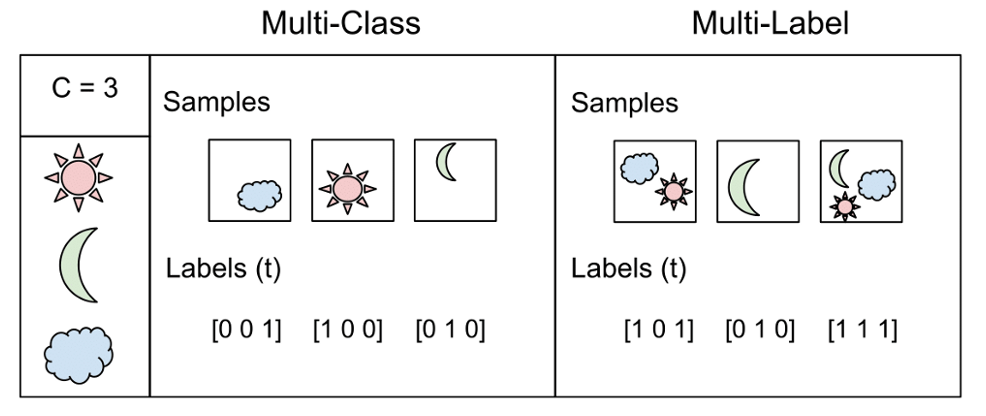
\includegraphics[width=0.6\linewidth]{Images/mlc.png}
        \caption*{\tiny Illustration of single-label vs multi-class vs multi-label classification. 
        From \url{https://medium.com/@wongsirikuln/fire-alert-system-with-multi-label-classification-model-explained-by-gradcam-bc18affe178c}.}
    \end{figure}
\end{frame}

%-------------------------------------------------

\begin{frame}{Background}
  \textbf{CNNs:} Three main types of layers:
  \begin{itemize}
    \item Convolutional layers: extract spatial features.
    \item Pooling layers: reduce dimensionality and summarise information.
    \item Fully Connected (FC) layer: interpret features for classification.
  \end{itemize}
\end{frame}

%-------------------------------------------------

\begin{frame}{Background}
  \textbf{Transformers:}
\end{frame}

%-------------------------------------------------

\begin{frame}{Background}
  \textbf{Vision Transformers (ViTs):}
\end{frame}

%-------------------------------------------------
\begin{frame}{Background}
  \begin{columns}
    \begin{column}{0.55\textwidth}
      \textbf{Loss functions}
      \begin{itemize}
        \item Measures distance between prediction (model output) and ground truth.
        \item Guides parameter optimization.
        \item Multi-label learning adds complexity: an image may trigger multiple simultaneous decisions.
        \item Choosing an appropriate loss is therefore important.
      \end{itemize}
    \end{column}

    \begin{column}{0.45\textwidth}
      \centering
      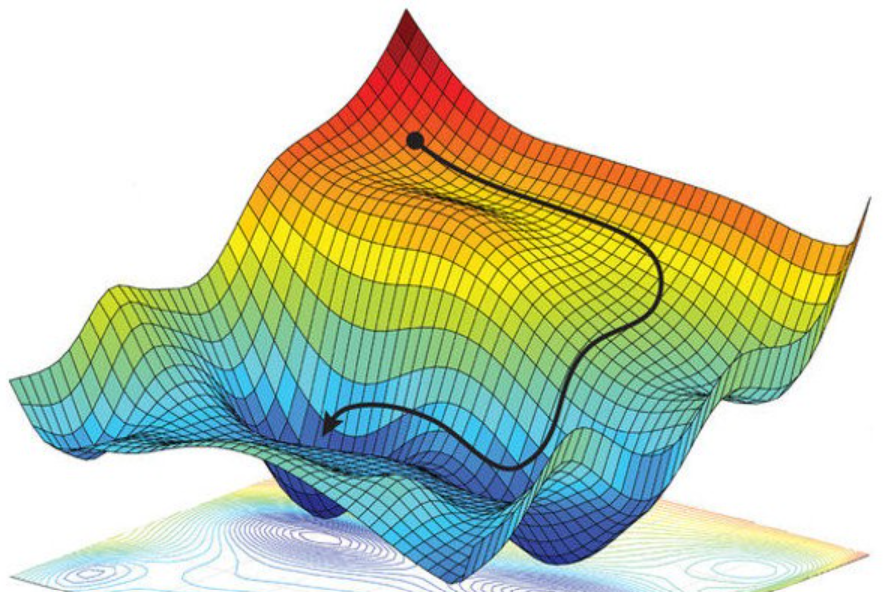
\includegraphics[width=0.9\linewidth]{Images/loss_optimization.png}\\
      \scriptsize Illustration of a loss landscape.
    \end{column}
  \end{columns}
\end{frame}

\begin{frame}{Background}
  \begin{columns}
    \begin{column}{0.55\textwidth}
      \textbf{Loss functions covered:}
          \begin{itemize}
            \item Binary Cross-Entropy (BCE)
            \item Expected Positive Regularisation (EPR)
            \item Regularised Online Label Estimation (ROLE)
            \item Focal and Asymmetric Focal Losses
          \end{itemize}
    \end{column}

    \begin{column}{0.45\textwidth}
      \centering
      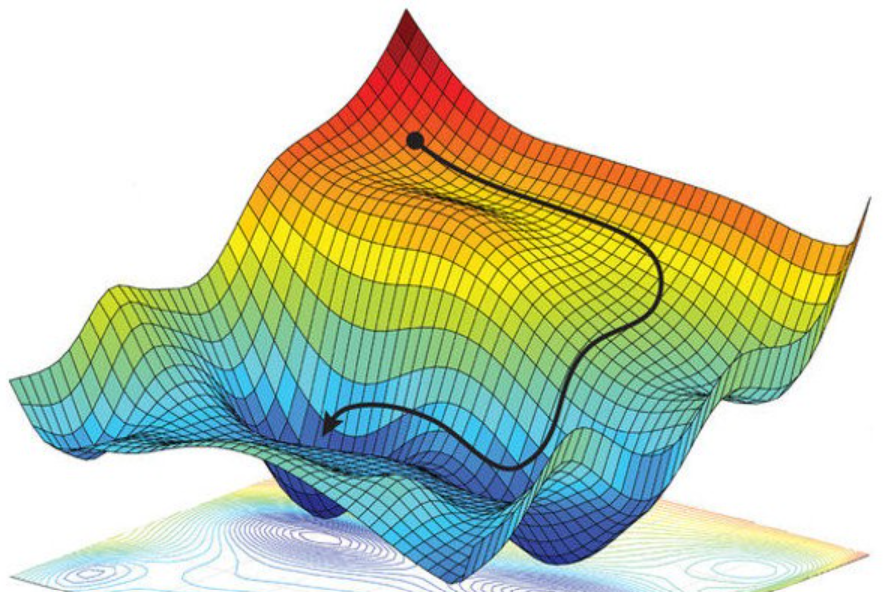
\includegraphics[width=0.9\linewidth]{Images/loss_optimization.png}\\
      \scriptsize Illustration of a loss landscape.
    \end{column}
  \end{columns}
\end{frame}

%-------------------------------------------------

\begin{frame}{Background}
\textbf{Binary Cross-Entropy (BCE):} 
  \begin{itemize}
    \item Independent positive/negative prediction per class: $y_i\in\{0,1\}$
    \item Model outputs probability $p_i \in [0,1]$ for each class $i\in\{1,\dots,K\}$.
  \end{itemize}
  \vspace{0.4em}
  \begin{equation*}
    \mathcal{L}_{\text{BCE}} = -\frac{1}{K}\sum_{i=1}^{K}\bigl[y_i\log p_i + (1-y_i)\log(1-p_i)\bigr]
  \end{equation*}
  % \begin{itemize}
  %   \item $K$: number of classes; $y_i\in\{0,1\}$, $p_i\in[0,1]$.
  %   \item Widely used baseline metric.
  % \end{itemize}
\end{frame}

%-------------------------------------------------

\begin{frame}{Background}
  \textbf{BCE limitations:}
\begin{itemize}
  \item \textbf{Class imbalance:} gradients dominated by frequent classes \textrightarrow{} rare classes under-represented.
  \item \textbf{Missing labels:} datasets rarely fully annotated. BCE treats unobserved labels as negatives, introducing false-negative bias.
\end{itemize}
  \vspace{0.5em}
  Positive-only BCE used when only the observed positive label $z_{ni}=1$ is known:
  \begin{equation*}
    \mathcal{L}_{\text{BCE}}^{+}(\mathbf{f}_n,\mathbf{z}_n) = - \sum_{i=1}^{K} \mathbf{1}[z_{ni}=1] \log f_{ni}
  \end{equation*}
\end{frame}

%-------------------------------------------------
\begin{frame}{Background}
  \textbf{Expected Positive Regularisation (EPR)}
    \begin{equation*}
      \mathcal{L}_{EPR}(\mathbf{F}_B,\mathbf{Z}_B) = \frac{1}{|B|}\sum_{n\in B}\mathcal{L}_{BCE}^+(\mathbf{f}_n,\mathbf{z}_n)+\lambda R_\kappa(\mathbf{F}_B)\text{,}
    \end{equation*}
  \begin{itemize}
    \item $\kappa$: expected positives per image (domain prior).
    \item $\hat{\kappa}$: average predicted positives in the batch.
    \item Batch penalty: $    R_\kappa(\mathbf{F}_B) = \left(\frac{\hat{\kappa}(\mathbf{F}_B)-\kappa}{K}\right)^2$.
  \end{itemize}
\end{frame}

% \begin{frame}{Background}
%   \textbf{Expected Positive Regularisation (EPR)}
% \begin{equation*}
% \mathcal{L}_{\text{EPR}}(\mathbf{F}_B,\mathbf{Z}_B)=\frac{1}{|B|}\sum_{n\in B}\mathcal{L}_{\text{BCE}}^{+}(\mathbf{f}_n,\mathbf{z}_n)+\lambda\bigl(\hat{\kappa}(\mathbf{F}_B)-\kappa\bigr)^{2}
% \end{equation*}
% \begin{itemize}
%   \item $\kappa$: expected positives per image (domain prior).
%   \item $\hat{\kappa}$: average predicted positives in the batch.
%   \item Penalises deviation from prior: mitigates false-positives when only few labels are observed.
% \end{itemize}
% \end{frame}

%-------------------------------------------------

\begin{frame}{Background}
  \textbf{Regularised Online Label Estimation (ROLE)}
  \begin{itemize}
    \item Jointly trains classifier $f(\cdot;\theta)$ and label-estimator $g(\cdot;\phi)$.
    \item Alternating updates:
      \[
        \mathcal{L}'(\mathbf{F}_B,\tilde{\mathbf{Y}}_B) = \frac{1}{|B|}\sum_{n\in B} \mathcal{L}_{BCE}(\mathbf{f}_n,\text{sg}(\tilde{\mathbf{y}}_n)) + \mathcal{L}_{EPR}(\mathbf{F}_B,\mathbf{Z}_B)
      \]
    \item Softly imputes missing labels ($0<y_{ni}<1$) and reduces false negatives.
  \end{itemize}
  \begin{equation*}
    \mathcal{L}_{ROLE}(\mathbf{F}_B, \mathbf{\tilde{Y}}_B) = \frac{\mathcal{L}'(\mathbf{F}_B|\mathbf{\tilde{Y}})+\mathcal{L}'(\mathbf{\tilde{Y}}|\mathbf{F}_B)}{2}
  \end{equation*}
\end{frame}

%-------------------------------------------------
\begin{frame}{Background}
  \textbf{Focal loss}
  \begin{equation*}
    \mathcal{L}_{\text{FL}} = -\frac{1}{K}\sum_{i=1}^{K}\alpha_i(1-p_i)^{\gamma}y_i\log p_i
  \end{equation*}

  \begin{itemize}
    \item Down-weights easy examples; focuses on hard, misclassified ones.
    \item Hyperparameters: focusing $\gamma$ and class weight $\alpha$.
  \end{itemize}
\end{frame}

%-------------------------------------------------
\begin{frame}{Background}
  \textbf{Assymetric focal loss}
  \begin{itemize}
    \item Variant tailored for imbalance in multi-label settings.
    \item Uses different focusing parameters for positive vs. negative terms.
  \end{itemize}
  \begin{equation*}
    \mathcal{L} = \frac{1}{K} \sum_{k=1}^{K}
    \begin{cases}
      (1 - p_k)^{\gamma^+} \log(p_k), & \text{if } y_k = 1 \\
      (p_k)^{\gamma^-} \log(1 - p_k), & \text{if } y_k = 0
    \end{cases}
  \end{equation*}
  % Typically $\gamma^+ < \gamma^-$. Encourages recall on rare classes while suppressing negatives.
\end{frame}

% \begin{frame}{Focal \& Asymmetric Focal Losses}
% \begin{itemize}
%   \item \textbf{Focal Loss (FL):} down--weights easy negatives, focuses on hard examples.
%     \[
%       \mathcal{L}_{\text{FL}} = -\frac{1}{K}\sum_{i=1}^{K}\alpha_i(1-p_i)^{\gamma}y_i\log p_i
%     \]
%   \item \textbf{Asymmetric Focal Loss (AFL):} separate focusing for positive/negative parts.
%     \[
%     \mathcal{L}_{\text{AFL}} = -\frac{1}{K}\sum_{i}\bigl[y_i(1-p_i)^{\gamma^{+}}\log p_i + (1-y_i)p_i^{\gamma^{-}}\log(1-p_i)\bigr]
%     \]
%   \item Useful when negatives hugely outnumber positives.
% \end{itemize}
% \end{frame}

%-------------------------------------------------

\begin{frame}{Key Take--aways}
\begin{itemize}
  \item BCE $\rightarrow{}$ solid baseline but fragile under imbalance and missing labels.
  \item EPR and ROLE repair missing--label bias with priors and online estimation.
  \item Focal variants tackle severe class imbalance.
  \item Choice of loss crucial for high multi--label performance (see results section).
\end{itemize}
\end{frame}

% \begin{frame}{Background}
%   \begin{columns}
%     \begin{column}{0.5\textwidth}
%       \textbf{Loss functions:}
%       \begin{itemize}
%         \item Binary Cross-Entropy (BCE)
%         \item Expected Positive Regularization (EPR)
%         \item Regularized Online Label Estimation (ROLE) 
%         \item Focal Loss
%         \item Asymmetric Focal Loss
%       \end{itemize}
%     \end{column}

%     \begin{column}{0.5\textwidth}
%        \begin{figure}
%         \centering
%         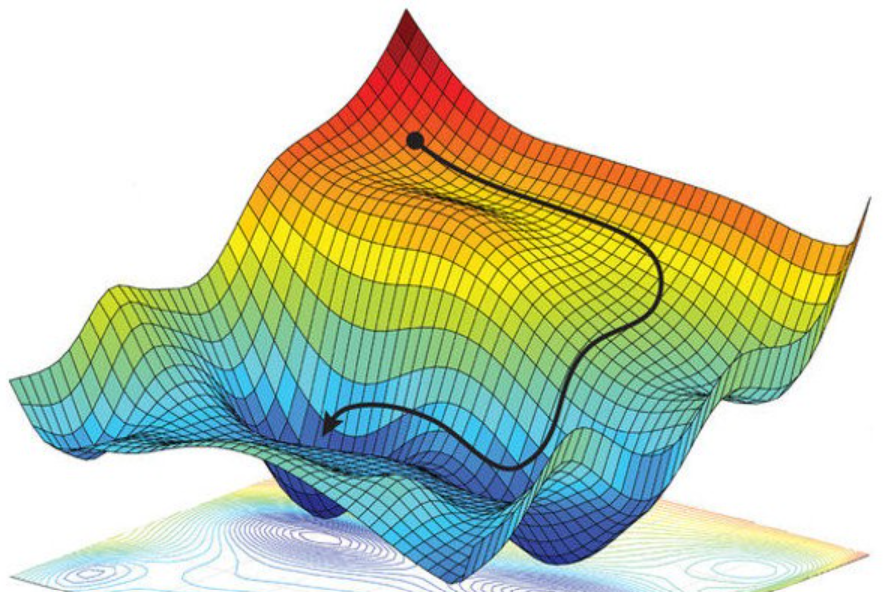
\includegraphics[width=0.9\linewidth]{Images/loss_optimization.png} 
%         \caption{Illustration of a loss landscape. From \url{https://ai.plainenglish.io/optimization-techniques-in-machine-learning-8b4f7325295}.} 
%       \end{figure}
%     \end{column}
%   \end{columns}
% \end{frame}

% %-------------------------------------------------

% \begin{frame}{Background}
%   \textbf{Binary Cross-Entropy (BCE):} 
%   \begin{itemize}
%     \item \textbf{Goal:} Classify data as either positive or negative (1 or 0).
%     \item \textbf{Output:} Probability score between 0 and 1
%   \end{itemize}

% \begin{equation*}
%   \mathcal{L}_{\text{BCE}} = -\frac{1}{K} \sum_{i=1}^{K} \bigl[ y_i\log(p_i) + (1-y_i)\log(1 - p_i) \bigr]
% \end{equation*}

%  where $K$ is the number of categories, $y_i\in[0,1]$ is the binary label, and $p_i$ is the predicted probability.
% \end{frame}

% \begin{frame}{Background}
%   \textbf{Binary Cross-Entropy (BCE):} 
%   \begin{itemize}
%     \item Popular benchmark for model performance in MLC.
%     \item Sensitive to class imbalance.
%     \item Assumes each training example is fully observable, leading to false negatives for partially observed labels.
%   \end{itemize}
% \end{frame}

% %-------------------------------------------------

% \begin{frame}{Background}
%   \textbf{Expected Positive Regularization (EPR):}

%   \begin{equation*}
%     \label{eq:epr}
%     \mathcal{L}_{EPR}(\mathbf{F}_B,\mathbf{Z}_B) = \frac{1}{|B|}\sum_{n\in B}\mathcal{L}_{BCE}^+(\mathbf{f}_n,\mathbf{z}_n)+\lambda R_\kappa(\mathbf{F}_B)\text{,}
% \end{equation*}
% \end{frame}

% %-------------------------------------------------

% \begin{frame}{Background}
%   \textbf{Regularized Online Label Estimation (ROLE):}
% \end{frame}

% %-------------------------------------------------

% \begin{frame}{Background}
%   \textbf{Focal loss:}
% \end{frame}

% %-------------------------------------------------

% \begin{frame}{Background}
%   \textbf{Asymmetric focal Loss:}
% \end{frame}

%-------------------------------------------------